% !TeX root = 2021-22-COMP110-09-workshop-materials-screen.tex
% Adjust these for the path of the theme and its graphics, relative to this file
%\usepackage{beamerthemeFalmouthGamesAcademy}
\usepackage{../../beamerthemeFalmouthGamesAcademy}
\usepackage{multimedia}
\graphicspath{ {../../} }

% Default language for code listings
\lstset{language=[Sharp]C
}

% For strikethrough effect
\usepackage[normalem]{ulem}
\usepackage{wasysym}

\usepackage{algpseudocode}

\usepackage{pdfpages}

% http://www.texample.net/tikz/examples/state-machine/
\usetikzlibrary{arrows,automata}
\usetikzlibrary{tikzmark,calc}

\newcommand{\modulecode}{COMP260}\newcommand{\moduletitle}{Distributed Systems}\newcommand{\sessionnumber}{5}

\begin{document}
\title{\sessionnumber: Data Structures II}
\subtitle{\modulecode: \moduletitle}

\frame{\titlepage} 

\begin{frame}{Worksheets Resume}
    \begin{center}
        Worksheet 6 is out now!

        Formative deadline: next Friday
    \end{center}
\end{frame}

%\part{2-dimensional arrays}
\frame{\partpage}

\begin{frame}{2-dimensional arrays}
	\pause Common problem: we want to represent a \textbf{2-dimensional array} of values (i.e.\ a grid)
	\pause
	$$
		\begin{matrix}
			v_{0,0} & v_{1,0} & \cdots & v_{w-1,0} \\
			v_{0,1} & v_{1,1} & \cdots & v_{w-1,1} \\
			\vdots  & \vdots  & \ddots & \vdots  \\
			v_{0,h-1} & v_{1,h-1} & \cdots & v_{w-1,h-1}
		\end{matrix}
	$$
\end{frame}

\begin{frame}{Approach 1: flat list}
	\begin{itemize}
		\pause\item For a $w \times h$ array, create a list of size $wh$
		\pause\item The element in column $x$ row $y$ is accessed by \lstinline{list[y * w + x]}
		\pause\item E.g.\ $w=5, h=4$:
		$$
			\begin{matrix}
				0 & 1 & 2 & 3 & 4 \\
				5 & 6 & 7 & 8 & 9 \\
				10 & 11 & 12 & 13 & 14 \\
				15 & 16 & 17 & 18 & 19
			\end{matrix}
		$$
	\end{itemize}
\end{frame}

\begin{frame}{Approach 2: list of lists}
	\begin{itemize}
		\pause\item For a $w \times h$ array, create a list of size $w$, where each element is a list of size $h$
			\begin{itemize}
				\pause\item Each element of the ``outer'' list represents a column of the array
			\end{itemize}
		\pause\item The element in column $x$ row $y$ is accessed by \lstinline{list[x][y]},
			i.e.\ the $y$th element of the $x$th column
	\end{itemize}
\end{frame}

\begin{frame}{Approach 3: dictionary}
	\begin{itemize}
		\pause\item Represent the array as a dictionary whose keys are \lstinline{(x,y)} tuples
		\pause\item The element in column $x$ row $y$ is accessed by \lstinline{list[x, y]}
	\end{itemize}
\end{frame}

\begin{frame}{Approach 4: NumPy array}
	\begin{itemize}
		\pause\item Requires NumPy or SciPy, and can only store numeric types
		\pause\item However, highly optimised for intensive calculations
			(e.g.\ ``tinkering'' with image pixel colours...?)
	\end{itemize}
\end{frame}

\begin{frame}{Which is best?}
	\begin{itemize}
		\pause\item Flat list is reasonably efficient but not very readable
		\pause\item List of lists is a reasonable trade-off between efficiency and readability
		\pause\item Dictionary allows for ``sparse'' arrays (e.g.\ some cells can be missing)
		\pause\item NumPy array is less versatile but faster in some use cases
	\end{itemize}
	\pause There is no single ``best'' approach --- it depends how you use it
\end{frame}

\part{Basic data structures in C\#}
\frame{\partpage}

\begin{frame}{Classes and interfaces}
    \begin{itemize}
        \pause\item A \textbf{class} in C\# defines constructors, destructor, methods, properties, fields, ...
        \pause\item An \textbf{interface} defines methods and properties which a class can implement
        \pause\item An interface is a little like a fully abstract class
        \pause\item A class in C\# can only \textbf{inherit} from one \textbf{class},
            but can \textbf{implement} several \textbf{interfaces}
    \end{itemize}
\end{frame}

\begin{frame}{IEnumerable}
    \begin{itemize}
        \pause\item Most container types in C\# implement the \lstinline{IEnumerable<ElementType>} interface
        \pause\item Anything implementing \lstinline{IEnumerable} can be iterated over with a \lstinline{foreach} loop
    \end{itemize}
\end{frame}

\begin{frame}[fragile]{Arrays}
    \begin{lstlisting}
int[] myArray = new int[10];
int[] anotherArray = new int[] { 123, 456, 789 };
    \end{lstlisting}
    \begin{itemize}
        \pause\item \lstinline{int[]} is an array of \lstinline{int}s
        \pause\item Size of the array is set on initialisation with \lstinline{new}
        \pause\item Array \textbf{cannot change size} after initialisation
        \pause\item Use \lstinline{myArray[i]} to get/set the \lstinline{i}th element (starting at 0)
        \pause\item Use \lstinline{myArray.Length} to get the number of elements
    \end{itemize}
\end{frame}

\begin{frame}[fragile]{Multi-dimensional arrays}
    \begin{lstlisting}
int[,] myGrid = new int[20, 15];
    \end{lstlisting}
    \begin{itemize}
        \pause\item \lstinline{int[,]} is an 2-dimensional array of \lstinline{int}s
        \pause\item Use \lstinline{myArray[x, y]} to get/set elements
        \pause\item Use \lstinline{myArray.GetLength(0)}, \lstinline{myArray.GetLength(1)} to get the ``width'' and ``height''
        \pause\item Similarly \lstinline{int[,,]} is a 3-dimensional array, etc.
    \end{itemize}
\end{frame}

\begin{frame}[fragile]{Lists}
    \begin{lstlisting}
using System.Collections.Generic;

List<int> myList = new List<int>();
List<int> anotherList = new List<int> { 1, 2, 3, 4 };
    \end{lstlisting}
	\begin{itemize}
		\pause\item Like a list in Python, but can only store values of the specified type (here \lstinline{int})
		\pause\item Has similar time complexity properties to Python lists
		\pause\item Append elements with \lstinline{myList.Add()}
		\pause\item Get the number of elements with \lstinline{myList.Count}
	\end{itemize}
\end{frame}

\begin{frame}[fragile]{Strings}
    \begin{lstlisting}
string myString = "Hello, world!";
    \end{lstlisting}
	\begin{itemize}
		\pause\item \lstinline{string} can be thought of as a container
		\pause\item In particular, it implements \lstinline{IEnumerable<char>}
	\end{itemize}
\end{frame}

\begin{frame}[fragile]{Strings are immutable}
	\begin{itemize}
		\pause\item Strings are \textbf{immutable} in C\#
        \pause\item This is also true in Python, but not in all programming languages
		\pause\item But wait... we change strings all the time, don't we?
	\end{itemize}
	\begin{lstlisting}
string myString = "Hello ";
myString += "world";
	\end{lstlisting}
	\begin{itemize}
		\pause\item This isn't changing the string, it's creating a new one and throwing the old one away!
		\pause\item Hence building a long string by appending can be slow (appending strings is $O(n)$)
		\pause\item C\# has a \textbf{mutable} string type: \lstinline{StringBuilder}
	\end{itemize}
\end{frame}

\begin{frame}{Dictionaries}
	\begin{itemize}
		\pause\item Dictionaries are \textbf{associative maps}
		\pause\item A dictionary maps \textbf{keys} to \textbf{values}
		\pause\item Takes two generic parameters: the \textbf{key type} and the \textbf{value type}
		\pause\item A dictionary is implemented as a \textbf{hash table}
	\end{itemize}		
\end{frame}

\begin{frame}[fragile]{Using dictionaries}
	\begin{lstlisting}
var age = new Dictionary<string, int> {
    ["Alice"] = 23,
    ["Bob"] = 36,
    ["Charlie"] = 27
};
	\end{lstlisting}
	\pause Access values using \lstinline{[]}:
	\begin{lstlisting}
Console.WriteLine(age["Alice"]);  // prints 23
age["Bob"] = 40;      // overwriting an existing item
age["Denise"] = 21;   // adding a new item
age.Add("Emily", 29); // adding a new item -- error if already present
	\end{lstlisting}
\end{frame}

\begin{frame}[fragile]{Iterating over dictionaries}
	\begin{itemize}
		\pause\item \lstinline{Dictionary<Key, Value>} implements \lstinline{IEnumerable<KeyValuePair<Key, Value>>}
		\pause\item \lstinline{KeyValuePair<Key, Value>} stores \lstinline{Key} and \lstinline{Value}
	\end{itemize}		
	\pause
	\begin{lstlisting}
foreach (var kv in age)
{
    Console.WriteLine("{0} is {1} years old", kv.Key, kv.Value);
}
	\end{lstlisting}
	\begin{itemize}
	    \pause\item (Note the \lstinline{var} keyword --- automatically determines the appropriate type to use for a variable)
		\pause\item Dictionaries are \textbf{unordered} --- avoid assuming that \lstinline{foreach}
		    will see the elements in any particular order!
	\end{itemize}		
\end{frame}

\begin{frame}{Hash sets}
	\begin{itemize}
		\pause\item Sets are \textbf{unordered} collections of \textbf{unique} elements
            \begin{itemize}
                \pause\item Sets \textbf{cannot} contain \textbf{duplicate} elements
                \pause\item Attempting to \lstinline{Add} an element already present in the set does nothing
            \end{itemize}
		\pause\item \lstinline{HashSet}s are like \lstinline{Dictionary}s without the values, just the keys
		\pause\item Certain operations on sets scale better on average than the equivalent operations on lists:
	\end{itemize}
	\pause
	\begin{center}
		\begin{tabular}{|c|c|c|}
			\hline
			\textbf{Operation} & \textbf{List} & \textbf{Hash Set} \\\hline
			Add element & Append: $O(1)$ & $O(1)$ \\
			& Insert: $O(n)$ & \\\hline
			Delete element & $O(n)$ & $O(1)$ \\\hline
			Contains element? & $O(n)$ & $O(1)$ \\\hline
		\end{tabular}
	\end{center}
\end{frame}

\begin{frame}[fragile]{Using sets}
	\begin{lstlisting}
var numbers = new HashSet<int>{1, 4, 9, 16, 25};
	\end{lstlisting}
	\pause Add and remove members with \lstinline{Add} and \lstinline{Remove} methods
	\begin{lstlisting}
numbers.Add(36);
numbers.Remove(4);
	\end{lstlisting}
	\pause Test membership with \lstinline{Contains}
	\begin{lstlisting}
if (numbers.Contains(9))
    Console.WriteLine("Set contains 9");
	\end{lstlisting}
\end{frame}

\newcommand{\socrative}{
	\begin{center}
		Socrative room code: \texttt{FALCOMPED}
	\end{center}
}

\part{Pass by reference}
\frame{\partpage}

\begin{frame}{References}
	\begin{itemize}
		\pause\item Our picture of a variable: a labelled box containing a value
		\pause\item For ``plain old data'' (e.g.\ numbers), this is accurate
		\pause\item For \textbf{objects} (i.e.\ instances of classes), variables actually hold
			\textbf{references} (a.k.a.\ \textbf{pointers})
		\pause\item It is possible (indeed common) to have \textbf{multiple references} to the same underlying object
	\end{itemize}
\end{frame}

\begin{frame}{The wrong picture}
	\begin{columns}
		\begin{column}{0.58\textwidth}
			\lstinputlisting{references_0.cs}
		\end{column}
		\pause
		\begin{column}{0.38\textwidth}
			\begin{center}
				\colorbox{white}{
					\color{black}
					\begin{tabular}{|c|c|}
						\hline
						\textbf{Variable} & \textbf{Value} \\\hline
						\texttt{x} & \uncover<3->{\begin{tabular}{|c|c|}
							\hline
							\texttt{a} & 30 \\\hline
							\texttt{b} & 40 \\\hline
						\end{tabular}} \\\hline
						\texttt{y} & \uncover<4->{\begin{tabular}{|c|c|}
							\hline
							\texttt{a} & 50 \\\hline
							\texttt{b} & 60 \\\hline
						\end{tabular}} \\\hline
						\texttt{z} & \uncover<5->{\begin{tabular}{|c|c|}
							\hline
							\texttt{a} & 50 \\\hline
							\texttt{b} & 60 \\\hline
						\end{tabular}} \\\hline
					\end{tabular}
				}
			\end{center}
		\end{column}
	\end{columns}
\end{frame}

\begin{frame}{The right picture}
	\begin{columns}
		\begin{column}{0.58\textwidth}
			\lstinputlisting{references_0.cs}
		\end{column}
		\pause
		\begin{column}{0.38\textwidth}
			\colorbox{white}{\parbox{0.9\textwidth}{
				\begin{center}
					\color{black}
					\begin{tabular}{|c|c|}
						\hline
						\textbf{Variable} & \textbf{Value} \\\hline
						\texttt{x} & \tikzmark{valuex} \\\hline
						\texttt{y} & \tikzmark{valuey} \\\hline
						\texttt{z} & \tikzmark{valuez} \\\hline
					\end{tabular}
					\par
					\vspace{3ex}
					\uncover<3->{\begin{tabular}{|c|c|}
						\hline
						\texttt{a} & \tikzmark{objectx}30 \\\hline
						\texttt{b} & 40 \\\hline
					\end{tabular}}
					\hspace{1ex}
					\uncover<4->{\begin{tabular}{|c|c|}
						\hline
						\texttt{a} & \tikzmark{objecty}50 \\\hline
						\texttt{b} & 60 \\\hline
					\end{tabular}}
				\end{center}
			}}
		\end{column}
	\end{columns}
	
\begin{tikzpicture}
		[
		  remember picture,
		  overlay,
		  -latex,
		  color=red,
		  yshift=0.5ex,
		  shorten >=1pt,
		  shorten <=1pt,
		]
		\pause\draw ({pic cs:valuex}) to [bend right] ($ ({pic cs:objectx}) + (0, 1ex) $);
		\pause\draw ({pic cs:valuey}) to [bend right] ($ ({pic cs:objecty}) + (0, 1ex) $);
		\pause\draw ({pic cs:valuez}) to [bend left] ($ ({pic cs:objecty}) + (0, 1ex) $);
	\end{tikzpicture}
\end{frame}

\begin{frame}{Values and references}
	\socrative
	\lstinputlisting{references_1.cs}
\end{frame}

\begin{frame}{Values and references}
	\socrative
	\lstinputlisting{references_2.cs}
\end{frame}

\begin{frame}{Values and references}
	\socrative
	\lstinputlisting{references_3.cs}
\end{frame}

\begin{frame}[fragile]{Pass by value}
	\socrative
	In \textbf{function parameters},
	``plain old data'' is passed by \textbf{value}
	\pause
	\begin{lstlisting}
void doubleIt(int x)
{
	x = x * 2;
}

int a = 7;
doubleIt(a);
Console.WriteLine(a);
	\end{lstlisting}
	\pause
	What does it print?
\end{frame}

\begin{frame}[fragile]{Pass by reference}
	\socrative
	However, objects (class instances) are passed by \textbf{reference}
	\pause
	\begin{lstlisting}
class Foo
{
	public int value;
	public Foo(int v) { value = v; }
}

void doubleIt(Foo x)
{
    x.value = x.value * 2;
}

Foo a = new Foo(7);
doubleIt(a);
Console.WriteLine(a.value);
	\end{lstlisting}
	\pause
	What does it print?
\end{frame}

\begin{frame}[fragile]{Lists are objects too}
	\pause
	\begin{lstlisting}
List<string> a = new List<string>{ "Hello" };
List<string> b = a;
b.Add("world");
foreach (string word in a)
{
	Console.WriteLine(word);
}
// Output:
//   Hello
//   world
\end{lstlisting}
	\pause
	... which means you should be careful when passing lists into functions,
	because the function might actually change the list!
\end{frame}

\begin{frame}[fragile]{Pass by value again}
	In C\#, struct instances are passed by \textbf{value}
	\pause
	\begin{lstlisting}
struct Foo
{
	public int value;
	public Foo(int v) { value = v; }
}

void doubleIt(Foo x)
{
    x.value = x.value * 2;
}

Foo a = new Foo(7);
doubleIt(a);
Console.WriteLine(a.value);
	\end{lstlisting}
	\pause
	This prints 7
\end{frame}

\begin{frame}{By reference or value?}
    \begin{itemize}
		\pause\item In C\#, these function arguments are passed \textbf{by value}:
			\begin{itemize}
				\pause\item Basic data types (\lstinline{int}, \lstinline{bool}, \lstinline{float} etc)
				\pause\item Instances of \lstinline{struct}s
			\end{itemize}
		\pause\item These function arguments are passed \textbf{by reference}:
			\begin{itemize}
				\pause\item Instances of \lstinline{class}es --- this includes classes built into .NET or Unity etc
				\pause\item Arguments with the \lstinline{ref} keyword attached
			\end{itemize}
		\pause\item Passing by value implies copying --- not a problem for small data values but beware of passing large structs around
    \end{itemize}
\end{frame}

\begin{frame}{References and pointers}
    \begin{itemize}
        \pause\item Some languages (e.g.\ C, C++) use \textbf{pointers}
        \pause\item Pointers are a type of reference, and have the same semantics
        \pause\item References in other languages (e.g.\ C\#, Python) are implemented using pointers
        \pause\item C++ also has something called references, which are similar but different
            (pointers can be \textbf{retargeted} whilst references cannot)
    \end{itemize}
\end{frame}

\begin{frame}{Pointers}
    \begin{itemize}
        \pause\item Recall that memory is a series of 1-byte locations, each with a numeric \textbf{address}
        \pause\item A \textbf{pointer} to something is simply the \textbf{address} at which it starts
        \pause\item When allocating a block of memory, the OS returns a pointer to the start of the block
        \pause\item When the memory is freed, any pointers into it are said to be \textbf{dangling}
        \pause\item If the memory is subsequently reused for something else, those pointers could end up
            pointing to random data
        \pause\item Again this is not really possible in Python/C\#, but a common source of bugs in C/C++
    \end{itemize}
\end{frame}

%\part{Generics in C\#}
\frame{\partpage}

\begin{frame}[fragile]{The problem}
    \begin{itemize}
        \pause\item Suppose we want to define a \lstinline{Pair} class to store two values
        \pause\item Something like this...
    \end{itemize}
    \pause
    \begin{lstlisting}
class PairOfInts
{
    public int first;
    public int second;
    
    public PairOfInts(int f, int s)
    {
        first = f;
        second = s;
    }
}
    \end{lstlisting}
\end{frame}

\begin{frame}[fragile]{The problem}
    \begin{itemize}
        \pause\item This is fine if we just want pairs of \lstinline{int}s
        \pause\item To store a pair of \lstinline{string}s we would need another class:
    \end{itemize}
    \pause
    \begin{lstlisting}
class PairOfStrings
{
    public string first;
    public string second;
    
    public PairOfStrings(string f, string s)
    {
        first = f;
        second = s;
    }
}
    \end{lstlisting}
\end{frame}

\begin{frame}[fragile]{The problem}
    \begin{itemize}
        \pause\item This quickly gets repetitive!
        \pause\item We could just store a pair of \lstinline{object}s --- in C\# \lstinline{object} can store values of any
            type
    \end{itemize}
    \pause
    \begin{lstlisting}
class PairOfObjects
{
    public object first;
    public object second;
    
    public PairOfObjects(object f, object s)
    {
        first = f;
        second = s;
    }
}
    \end{lstlisting}
    \begin{itemize}
        \pause\item However this doesn't let us impose type safety
    \end{itemize}
\end{frame}

\begin{frame}[fragile]{The solution}
    \begin{itemize}
        \pause\item \textbf{Generics} are a feature of C\# which let us pass types as ``parameters''
    \end{itemize}
    \pause
    \begin{lstlisting}
class Pair<ElementType>
{
    public ElementType first;
    public ElementType second;
    
    public PairOfObjects(ElementType f, ElementType s)
    {
        first = f;
        second = s;
    }
}
    \end{lstlisting}
    \begin{itemize}
        \pause\item \lstinline{ElementType} can be any type
    \end{itemize}
\end{frame}

\begin{frame}[fragile]{The solution}
    \begin{itemize}
        \pause\item When we instantiate the generic class, we pass in the type in angle brackets:
    \end{itemize}
    \pause
    \begin{lstlisting}
Pair<int> pairOfInts = new Pair<int>(12, 34);
Pair<string> pairOfStrings = new Pair<string>("hello", "world");
    \end{lstlisting}
\end{frame}

\begin{frame}[fragile]{Multiple parameters}
    \begin{itemize}
        \pause\item Generics can take multiple parameters:
    \end{itemize}
    \pause
    \begin{lstlisting}
class Pair<Type1, Type2>
{
    public Type1 first;
    public Type2 second;
    
    public PairOfObjects(Type1 f, Type2 s)
    {
        first = f;
        second = s;
    }
}
    \end{lstlisting}
    \begin{lstlisting}
Pair<int, string> x = new Pair<int, string>(123, "hello");
    \end{lstlisting}
\end{frame}

\begin{frame}{Why generics?}
    \begin{itemize}
        \pause\item Generics let us write type safe code which can be adapted to data of different types
        \pause\item Standard libraries in .NET and Unity make use of generics for e.g.\ container types
        \pause\item Similar to \textbf{templates} in C++
    \end{itemize}
\end{frame}


\part{More data structures}
\frame{\partpage}

\begin{frame}{Stacks and queues}
	\begin{columns}
		\pause
		\begin{column}{0.3\textwidth}
			
\includegraphics[width=\textwidth]{stack}
		\end{column}
		\begin{column}{0.68\textwidth}
			\begin{itemize}
				\item A \textbf{stack} is a \textbf{last-in first-out (LIFO)} data structure
				\pause\item Items can be \textbf{pushed} to the \textbf{top} of the stack
				\pause\item Items can be \textbf{popped} from the \textbf{top} of the stack
			\end{itemize}
		\end{column}
	\end{columns}
	\begin{columns}
		\pause
		\begin{column}{0.3\textwidth}
			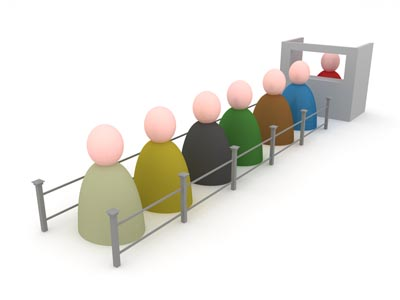
\includegraphics[width=\textwidth]{queue}
		\end{column}
		\begin{column}{0.68\textwidth}
			\begin{itemize}
				\item A \textbf{queue} is a \textbf{first-in first-out (LIFO)} data structure
				\pause\item Items can be \textbf{enqueued} to the \textbf{back} of the queue
				\pause\item Items can be \textbf{dequeued} from the \textbf{front} of the queue
			\end{itemize}
		\end{column}
	\end{columns}
\end{frame}

\begin{frame}{Stacks and queues in Python}
	\begin{itemize}
		\pause\item Stacks can be implemented efficiently as lists
		\pause\item Queues can be implemented as lists, but not efficiently
		\pause\item \lstinline{deque} (from the \lstinline{collections} module) implements an efficient
			\textbf{double-ended queue}
		\pause\item Inserting and removing elements from the start and end of a \lstinline{deque} is $O(1)$
	\end{itemize}
\end{frame}

\begin{frame}{Graphs}
	\begin{columns}
		\pause
		\begin{column}{0.3\textwidth}
			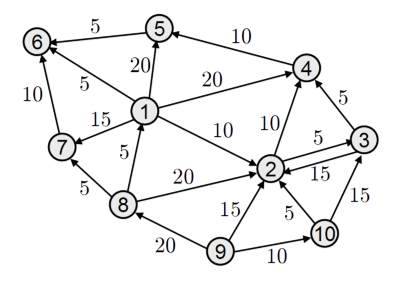
\includegraphics[width=\textwidth]{graph1}
			\par
			\vspace{2ex}
			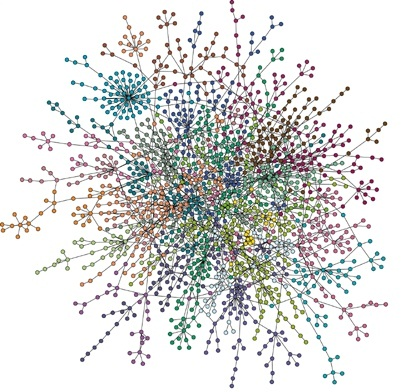
\includegraphics[width=\textwidth]{graph2}
		\end{column}
		\begin{column}{0.68\textwidth}
			\begin{itemize}
				\pause\item A \textbf{graph} is defined by:
					\begin{itemize}
						\pause\item A collection of \textbf{nodes} or \textbf{vertices} (points)
						\pause\item A collection of \textbf{edges} or \textbf{arcs} (undirected lines or directed arrows between points)
					\end{itemize}
				\pause\item Often used to model \textbf{networks} (e.g.\ social networks, transport networks, game levels, finite state automata, ...)
			\end{itemize}
		\end{column}
	\end{columns}
\end{frame}

\begin{frame}{Trees}
	\begin{columns}
		\pause
		\begin{column}{0.3\textwidth}
			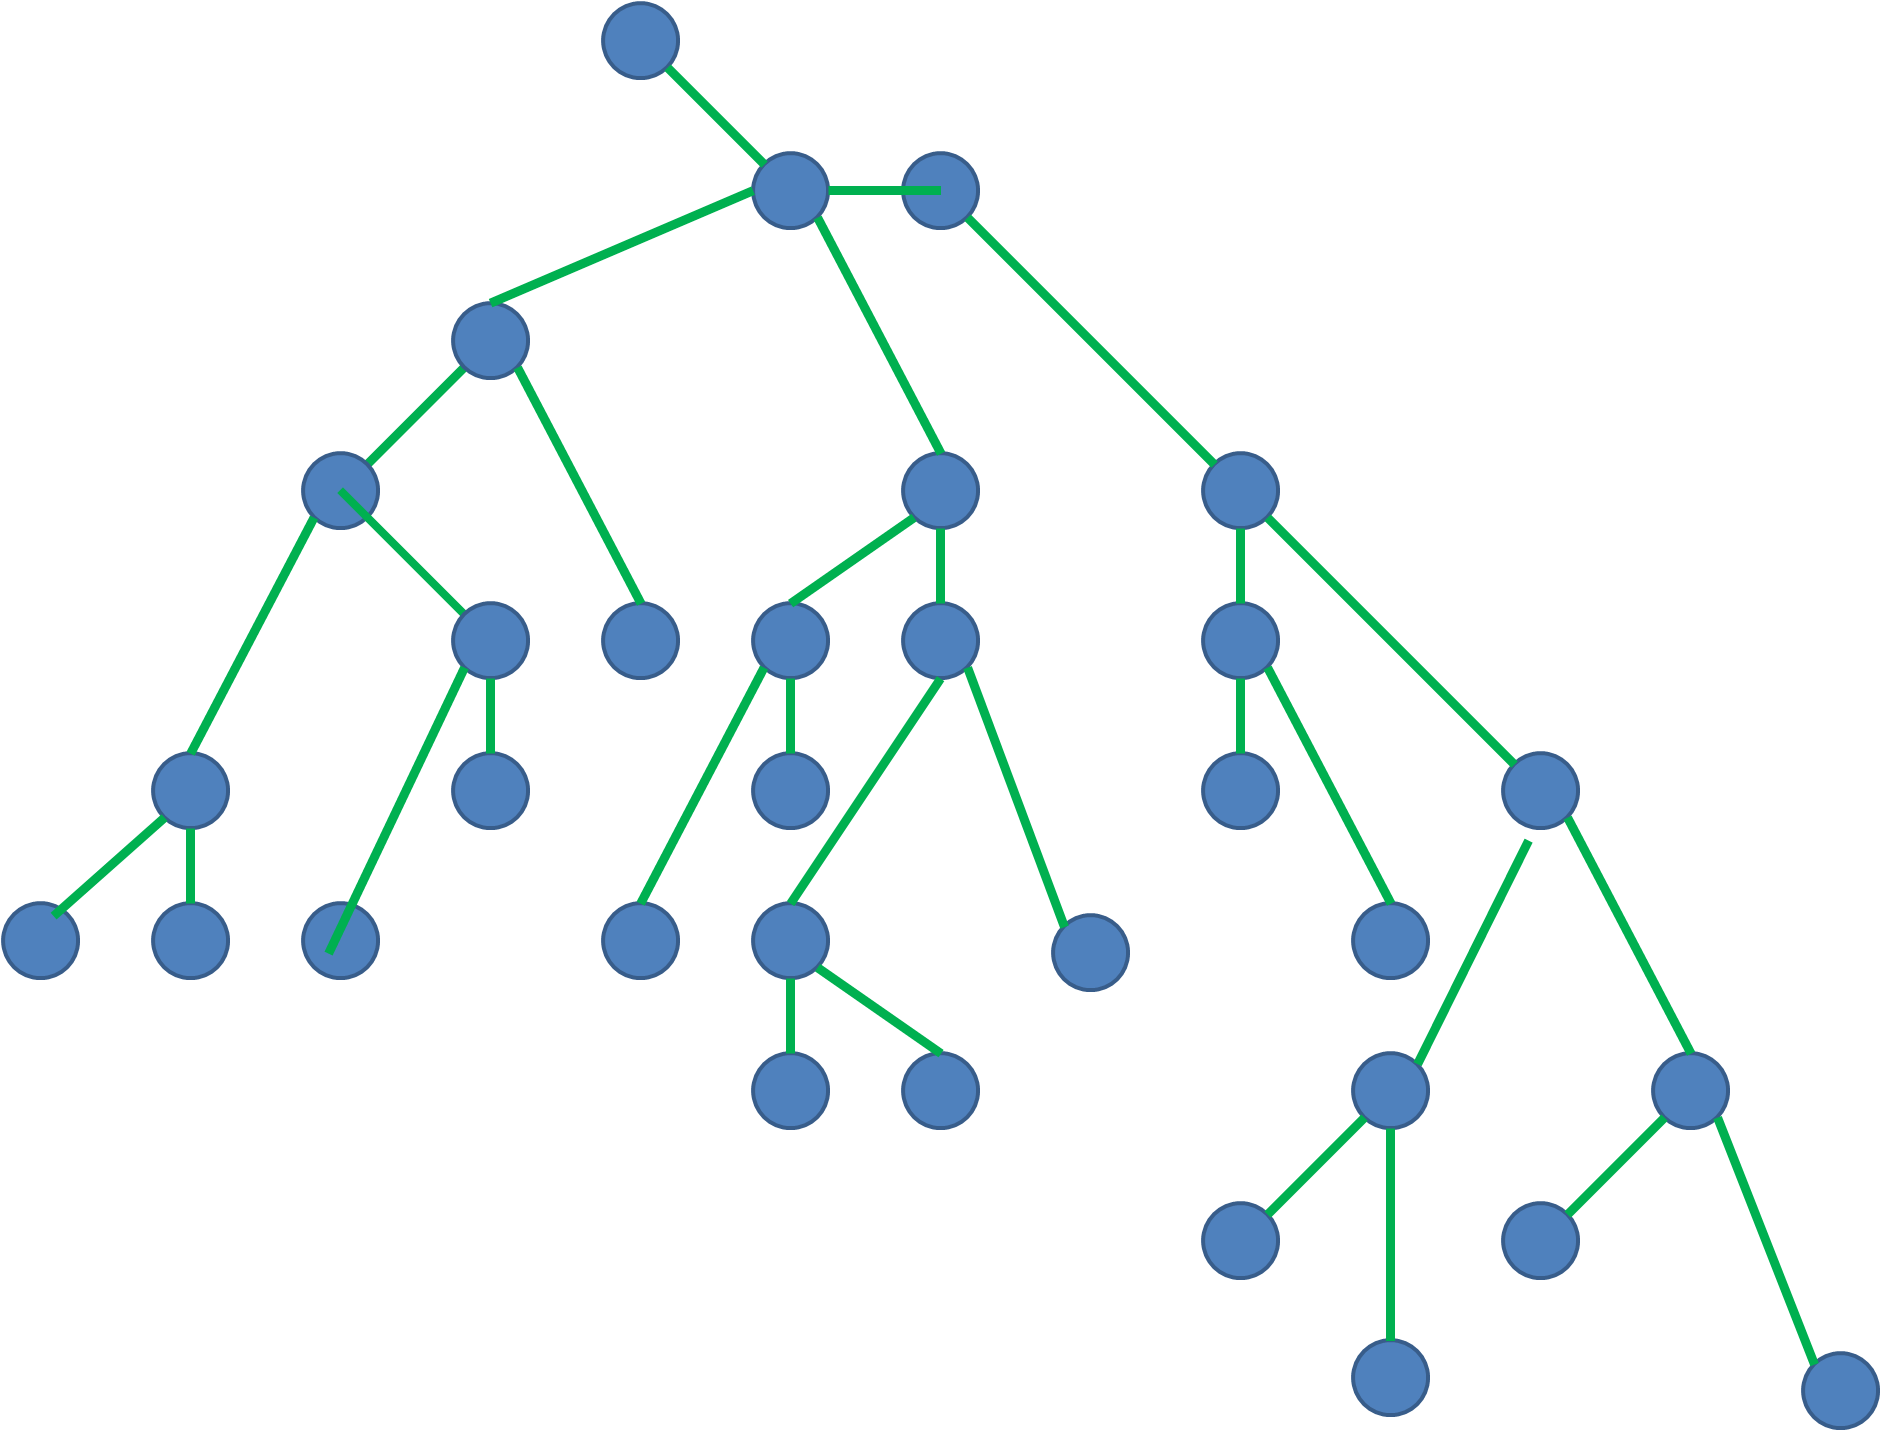
\includegraphics[width=\textwidth]{tree2}
			\par
			\vspace{2ex}
			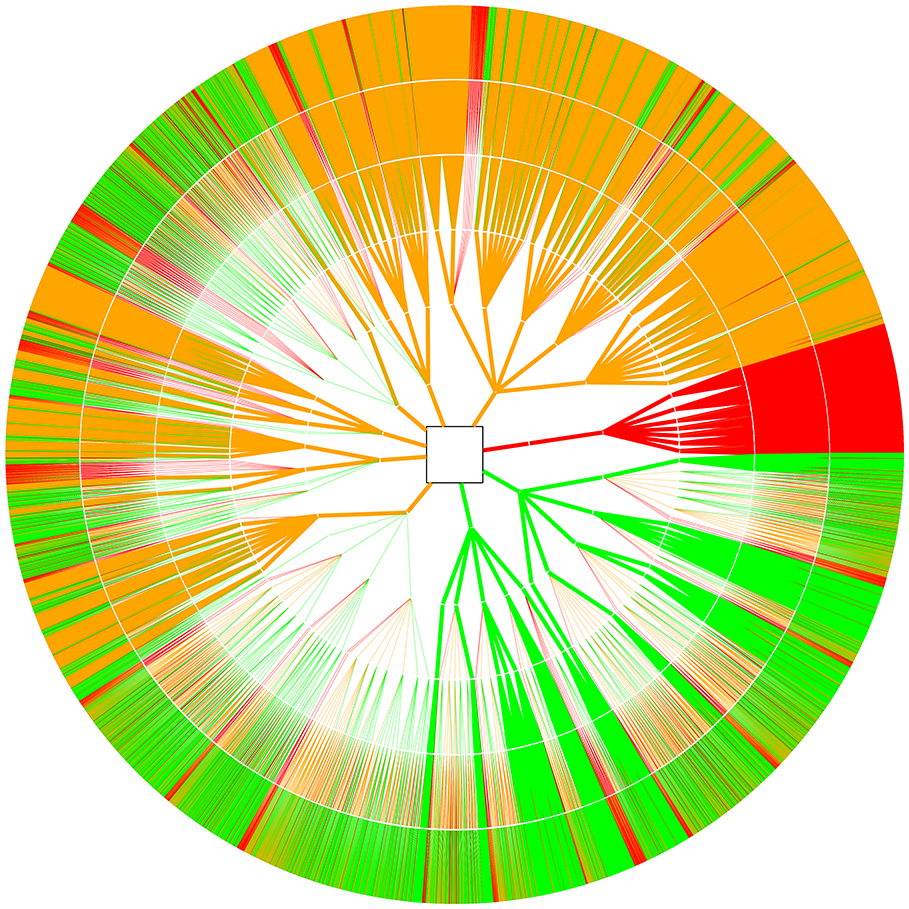
\includegraphics[width=\textwidth]{tree}
		\end{column}
		\begin{column}{0.68\textwidth}
			\begin{itemize}
				\pause\item A \textbf{tree} is a special type of directed graph where:
					\begin{itemize}
						\pause\item One node (the \textbf{root}) has no incoming edges
						\pause\item All other nodes have exactly 1 incoming edge
					\end{itemize}
				\pause\item Edges go from \textbf{parent} to \textbf{child}
					\begin{itemize}
						\pause\item All nodes except the root have exactly one parent
						\pause\item Nodes can have 0, 1 or many children
					\end{itemize}
				\pause\item Used to model \textbf{hierarchies} (e.g.\ file systems, object inheritance, scene graphs, state-action trees, ...)
			\end{itemize}
		\end{column}
	\end{columns}
\end{frame}


%\part{Linked lists}
\frame{\partpage}

\begin{frame}{Linked list}
	\begin{itemize}
		\pause\item Composed of a number of \textbf{nodes}
		\pause\item Each node contains:
			\begin{itemize}
		 		\pause\item An \textbf{item} --- the actual data to be stored
		 		\pause\item A pointer or reference to the \textbf{previous node} in the list (null for the first item)
		 		\pause\item A pointer or reference to the \textbf{next node} in the list (null for the last item)
			\end{itemize}
	\end{itemize}
	\pause
	\vspace{2ex}
	\begin{center}
	    \setlength{\tabcolsep}{0.2em}
		\begin{tabular}{|c|c|c|}
			\hline
			{\tiny prev} & {\tiny item} & {\tiny next} \\
			$\times$ & \texttt{\footnotesize first} & \tikzmark{nexta} \\\hline
		\end{tabular}
		\qquad
		\begin{tabular}{|c|c|c|}
			\hline
			{\tiny prev} & {\tiny item} & {\tiny next} \\
			\tikzmark{prevb} & \texttt{\footnotesize second} & \tikzmark{nextb} \\\hline
		\end{tabular}
		\qquad
		\begin{tabular}{|c|c|c|}
			\hline
			{\tiny prev} & {\tiny item} & {\tiny next} \\
			\tikzmark{prevc} & \texttt{\footnotesize third} & $\times$ \\\hline
		\end{tabular}
		
\begin{tikzpicture}
			[
			  remember picture,
			  overlay,
			  -latex,
			  yshift=0.5ex,
			  shorten >=1pt,
			  shorten <=1pt,
			]
			\draw ($ ({pic cs:nexta}) + (0, 0.5ex) $) to ($ ({pic cs:prevb}) + (-1.2ex, 0.5ex) $);
			\draw ($ ({pic cs:nextb}) + (0, 0.5ex) $) to ($ ({pic cs:prevc}) + (-1.2ex, 0.5ex) $);
			\draw ($ ({pic cs:prevb}) + (0, -0.5ex) $) to ($ ({pic cs:nexta}) + (1.2ex, -0.5ex) $);
			\draw ($ ({pic cs:prevc}) + (0, -0.5ex) $) to ($ ({pic cs:nextb}) + (1.2ex, -0.5ex) $);
		\end{tikzpicture}
	\end{center}
\end{frame}

\newcommand{\footnoteref}[1]{$^{\text{\ref{#1}}}$}

\begin{frame}{Linked lists vs arrays}
	\begin{center}
		\begin{tabular}{|r|l|l|}
			\hline
			\textbf{Operation} & \textbf{Array} & \textbf{Linked list} \\\hline
			\pause Append & $O(1)$ & $O(1)$ \footnote{\label{f:llend}If we already have a reference to the last node} \\
			\pause Pop & $O(1)$ & $O(1)$ \footnoteref{f:llend} \\
			\pause Index lookup & $O(1)$ & $O(n)$ \\
			\pause Count elements & $O(1)$ & $O(n)$ \\
			\pause Insert & $O(n)$ & $O(1)$ \footnote{\label{f:llinsert}If we already have a reference to the relevant node} \\
			\pause Delete & $O(n)$ & $O(1)$ \footnoteref{f:llinsert} \\
			\hline
		\end{tabular}
	\end{center}
\end{frame}

\begin{frame}{Implementing a linked list}
\end{frame}

%\part{Workshop}
\frame{\partpage}

% \begin{frame}{Workshop}
%     \footnotesize
%     \begin{columns}
%         \begin{column}{0.45\textwidth}
%             For each of the following collections:
            
%                 array, \lstinline{List}, \lstinline{LinkedList},
%                 \lstinline{Dictionary}, \lstinline{HashSet},
%                 \lstinline{SortedDictionary}, \lstinline{SortedList},
%                 \lstinline{SortedSet}, \lstinline{Stack}, \lstinline{Queue}
                
%             And each of the operations $\to$, use the Microsoft .NET documentation
%             and experimentation to answer the following:
            
%             \begin{itemize}
%                 \item Does this operation make sense / is it possible?
%                 \item If so, how do you do it?
%                 \item What is the time complexity?
%             \end{itemize}
%         \end{column}
%         \begin{column}{0.55\textwidth}
%             \begin{itemize}
%                 \item Add an element at the [beginning, $i$, end]
%                 \item Remove an element at the [beginning, $i$, end]
%                 \item Get the [first, $i$th, last] element
%                 \item Find if a specific element is present
%                 \item Get the [smallest, largest] element
%                 \item Get the number of elements
%                 \item Copy the collection
%                 \item Reverse the collection
%                 \item Sort the collection
%                 \item Randomly shuffle the collection
%                 \item Print a string listing the contents
%             \end{itemize}
%         \end{column}
%     \end{columns}
% \end{frame}

\begin{frame}{Workshop Activity}
    \begin{itemize}
        \pause\item \textbf{Priority 1}: check you have submitted your research journal!
        \pause\item Then, in your \textbf{breakout groups} (from week 2 on LearningSpace):
        \pause\item I have put a Word document in your room on Teams (Files tab) --- you can edit this collaboratively
        \pause\item For a variety of C\# collection types:
            \begin{itemize}
                \pause\item What operations are possible?
                \pause\item How are they done?
                \pause\item What is their time complexity?
                \pause\item What is an example scenario where this data structure is appropriate?
            \end{itemize}
        \pause\item Use the \textbf{Microsoft .NET documentation} along with \textbf{googling} and \textbf{experimentation} to find out!
        \pause\item Reconvene here at \textbf{5:30pm} to compare notes
    \end{itemize}
\end{frame}


\part{Workshop}
\frame{\partpage}

\begin{frame}{Workshop}
    \begin{center}
        Begin working on Worksheet 6

        I am available for the rest of the session if you run into any problems!

        (Or if you have any general questions etc.)
    \end{center}
\end{frame}


\end{document}
